\section{Hypothesis Graph}
\label{section: hgraph}
When given a task the hypothesis graph starts generating action sequences, to give an overview of how such action sequences are generated, \cref{figure: flowchart_hgraph} was created. An HGraph can start generating hypothesises or action sequences when a task and the environment are provided. The HGraph alternates between executing and replanning to complete the task. \\

\newpage
\begin{figure}[H] 
\begin{tikzpicture}[node distance = 3cm]
    % Nodes
    \node [block, fill=yellow!50, line width=2pt, dashed] (first) {create start and target node};
    
    % legend
    \node[text width=2.8cm, yshift=1cm, right of=first, node distance=7cm, text centered, rounded corners, minimum height=1em, label={[name=lab, yshift=0.4cm, left]\textbf{Legend}}] (legend1) {\small Update KGraph};
    \node[rectangle, draw, left of=legend1, fill=green!50, rounded corners, minimum height=1em, minimum width=1cm, node distance=2cm] (legend1color) {};
    
    \node[text width=2.8cm, below of=legend1, text centered, minimum height=1em, node distance=0.7cm] (legend2) {\small Query KGraph};
    \node[rectangle, draw, left of=legend2, fill=red!40, rounded corners, minimum height=1em, minimum width=1cm, node distance=2cm] (legend2color) {};
   
    \node[text width=2.8cm, below of=legend2, text centered, minimum height=1em, node distance=0.7cm] (legend3) {\small Update C-Space};
    \node[rectangle, draw, left of=legend3, fill=yellow!50, rounded corners, minimum height=1em, minimum width=1cm, node distance=2cm] (legend3color) {};
    
    \node[text width=2.8cm, below of=legend3, text centered, minimum height=1em, node distance=0.7cm] (legend4) {\small action in HGraph};
    \node[rectangle, draw, left of=legend4, rounded corners, minimum height=1em, minimum width=1cm, node distance=2cm, line width=2pt, dashed] (legend4color) {};
 
    \node[text width=2.8cm, below of=legend4, text centered, minimum height=1em, node distance=0.7cm] (legend5) {\small action in C-Space};
\node[rectangle, draw, left of=legend5, rounded corners, minimum height=1em, minimum width=1cm, node distance=2cm, line width=2pt] (legend5color) {};

    % nodes, Path exists 
    \node [decision, below of=first, node distance=3cm, line width=2pt] (path_existence) {Path non-existence};
    \node [decision, left of=path_existence, node distance=4.5cm, line width=2pt, dashed] (subtasks) {Is there a Subtask};
    \node [block, above of=subtasks, node distance=2.7cm] (no_solution_found) {no solution found};
    
    % nodes, Knowledge available
    \node [decision, fill=red!40, below of=path_existence, node distance=3cm, inner sep=0.5mm] (know_avail) { Knowledge Available };
    \node [decision, fill=red!40, right of=know_avail, node distance=3.5cm, inner sep=0.5mm] (know_good) {Knowledge Usable};
    \node [decision, right of=know_good, node distance=3.5cm, inner sep=0.5mm] (movable) {Obstacle Movable or Unkown};
    \node [block, left of=know_avail, node distance=3cm, line width=2pt, dashed] (impossible) {impossible task, abort subtask};
    
    % nodes, Generate new transition
    \node [decision, below of=know_avail, node distance=3.2cm, line width=2pt, inner sep=0.5mm, dashed] (goto_sys_iden) {Generate new Transition};
    \node[block, right of=goto_sys_iden, node distance=3.5cm, line width=2pt, dashed] (no_trans_found) {no transaction found, abort subtask};
    
    
    % Motion/Manipulation planning 
    \node [decision, below of=goto_sys_iden, node distance=3.5cm] (single_multi) {Single, Multi- body};
    \node [decision, line width=2pt, dashed, left of=single_multi, node distance=3.7cm] (model_avail_single) {Model available};
    \node [decision, line width=2pt, dashed, right of=single_multi, node distance=3.7cm] (model_avail_multi) {Model available};
    \node [block, line width=2pt, dashed, left of=model_avail_single, node distance=2.7cm] (sys_iden_single) {Add subtask Sys. Iden.};
    \node [block, line width=2pt, dashed, right of=model_avail_multi, node distance=3cm] (sys_iden_multi) {Add subtasks Go To + Sys. Iden.};
    \node [block, line width=2pt, dashed, below of=single_multi, node distance=3cm] (move_object) {Add subtask to Move Object};
    \node [block, line width=2pt, left of=move_object, node distance=3.7cm] (motion_planning) {Motion Planning};
    \node [block, line width=2pt, right of=move_object, minimum width=2.3cm, node distance=3.7cm] (manipulation_planning) {Manipulation Planning};
    
    % nodes, Path to target
    \node [decision, below of =move_object, node distance=3.5cm, line width=2pt, dashed] (global_path) {Path to Target}; 
    \node [decision, right of=global_path, node distance=3.5cm, line width=2pt, dashed] (first_action) {First Action Planned};
    \node [decision, right of=first_action, diagonal fill={yellow!50}{green!50}, node distance=3cm] (execute) {Execute};
     
    % nodes, Target node reached 
    \node [decision, below of=global_path, node distance=3cm, line width=2pt, dashed] (target_node_reached) {Target Node Reached};
    \node [block, left of=target_node_reached, node distance=3cm] (end) {Task successfully executed};
    
    % Edges
    \path[line] ++(0,1.5) -- node[left]{task} (first);
    \path[line] (first) -- node[midway](to_path_exists){}(path_existence); 
    
    % edges, Path exists 
    \path[line] (path_existence) -- node[midway, above, left] {no} (impossible.north east);
    \path[line] (subtasks.north) --  node[left] {no} (no_solution_found);
    \path[line] (path_existence) -- node[left] {yes} (know_avail); 
    \path[line] (subtasks.east) -- node[above] {yes} (path_existence.west);
    
    % edges, Knowledge available
    \path[line] (know_avail) -- node[above] {yes} (know_good); 
    \path[line] (know_avail) -- node[left](toward_new_trans) {no} (goto_sys_iden); 
    \draw[->] (know_good.east) -- node[above] {yes} (movable.west);
    
    % \draw[-]  ([xshift=3.2mm]toward_new_trans.center) -| node[near start, above] {no} (know_good.south);
    \draw[-](impossible.west) -- +(-0.47,0); 
     
    \draw[->]  ([xshift=1.75cm, yshift=7.7cm]know_avail.center) --  node[at start, above] {action suggestions} ([xshift=1.75cm, yshift=1.75cm]know_avail.center) -- (know_avail.north east);
    \draw[->]  ([xshift=1.75cm, yshift=1.75cm]know_avail.center) -- (know_good.north west);
    \draw [draw=white,double distance=\pgflinewidth,ultra thick] (path_existence.east) -- +(2cm,0);
    
    % edges, Generate new transition
    \draw[-] (move_object.south) |- +(-8.2,-0.3);
    \draw [draw=white,double=black,double distance=\pgflinewidth,ultra thick] (motion_planning.south) -- +(0,-1cm);
    \draw[-stealth] (motion_planning.south)  -- ([yshift=-1cm]motion_planning.south) -| node[near start, above] {success} (global_path.north);
    \draw[-] (manipulation_planning.south) -- ([yshift=-1cm]manipulation_planning.south) -| node[near start, above] {success} (global_path.north);
    \draw[-] (motion_planning.west) -- node[above] {failure} +(-3.47,0);
    \draw[-] (manipulation_planning.east) -| node[near start, above] {failure} ([xshift=4.7cm,yshift=-0.6cm]no_trans_found.south) -- ([yshift=-0.6cm]no_trans_found.south);
    
    % edges, Single/Multi body
    \draw[-stealth] (single_multi.west) -- node[above] {single} (model_avail_single);
    \draw[-stealth] (single_multi.east) -- node[above] {multi} (model_avail_multi);
    \draw[-stealth] (model_avail_single.south) -- node[left] {yes} (motion_planning.north);
    \draw[-stealth] (model_avail_single.west) -- node[above] {no} (sys_iden_single);
    \draw[-stealth] (model_avail_multi.south) -- node[near start, left] {yes} (manipulation_planning.north);
    \draw[-stealth] (model_avail_multi.east) -- node[above] {no} (sys_iden_multi);
    \draw[-stealth] (motion_planning.east) -- node[above] {blockade} (move_object);
    \draw[-stealth] (manipulation_planning.west) -- node[above] {blockade} (move_object);
    \draw[-stealth] (goto_sys_iden) -- node[above] {failure} (no_trans_found);
    \draw[-] (sys_iden_single.north) --  ([yshift=1.07cm]sys_iden_single.north);
    \draw[-] (sys_iden_multi.north) |-  ([yshift=-0.6cm]no_trans_found.south);
    \draw[-] (no_trans_found.south) -- ++(0,-0.6cm) --([xshift=-8cm, yshift=-0.6cm]no_trans_found.south);
    \draw [draw=white,double=black,double distance=\pgflinewidth,ultra thick] (goto_sys_iden.south) -- node[at start, left] {success}(single_multi.north);
    \draw[-stealth] ([yshift=-0.5cm]goto_sys_iden) -- (single_multi.north);
    
    \draw[-] (movable.south) |- node[near start, left] {yes} ([xshift=-1.5cm, yshift=-1.4cm]movable.south) |- ([yshift=0.2cm]single_multi.north);
    \draw [draw=white,double distance=\pgflinewidth,ultra thick]  (movable.north) |- ([xshift=-8cm, yshift=0.1cm]movable.north);
    \draw[-] (movable.north) |- node[above]{no}([xshift=-8.08cm, yshift=0.1cm]movable.north);
    % HERE
    \draw [draw=white,double=black,double distance=\pgflinewidth,ultra thick] ([xshift=5.5cm,yshift=0.3cm]single_multi.north) -- ([xshift=5.5cm, yshift=2cm]single_multi.north);
    % \draw[-] (know_good.east) -| node[above]{yes} ([xshift=5.5cm, yshift=0.2cm]single_multi.north) -- ([yshift=0.2cm]single_multi.north);
    
    % edges, Path to target
    \path[line] (global_path) -- node[above] {yes} (first_action);
    \path[line] (first_action.east) -- node[above] {yes} (execute);
    \path[line] (global_path.west) -| node[left, below, near start] {no} ([xshift=-7cm, yshift=8.31cm]global_path.west) -|  (subtasks.south); 
   
    \draw[-stealth] (first_action.north) |- node[near end, above] {no} ([xshift=1.7cm, yshift=0.15cm]first_action.north) |- ([yshift=-0.35cm]single_multi.south) -- (single_multi.south);
    \draw [draw=white,double=black,double distance=\pgflinewidth,ultra thick] (manipulation_planning.east) -- +(1cm,0);
    \draw [draw=white,double=black,double distance=\pgflinewidth,ultra thick] (manipulation_planning.north) -- +(0,1cm);
    
    \draw[-stealth] ([yshift=0.2cm, xshift=0.2cm]execute.south east) --  ([yshift=-0.8cm, xshift=1.2cm]execute.south east) -- node[at end, left] {robot input, action feedback} +(0,-2.7cm);
    
    \draw[stealth-] ([yshift=-0.2cm, xshift=-0.2cm]execute.south east) --  ([yshift=-1.2cm, xshift=0.8cm]execute.south east) -- node[left, at end] {sensor measurements} +(0, -1.8cm);
    
    \path[line] (execute.south) |- node[near start, left] {success} (target_node_reached.east);
    \draw[-stealth] (execute.east) -- node[above] {failure} ([xshift=1.5cm]execute.east) |- (path_existence.east);
    
    
    % edges, Target node reached 
    \path[line] (target_node_reached.north) -- node[left] {no} (global_path.south);
    \path[line] (target_node_reached.west) -- node[above] {yes} (end.east);

\end{tikzpicture}
\caption{Flowchart displaying the hypothesis graph's workflow.}
\label{figure: flowchart_hgraph} 
\end{figure}

\subsection{Definition}
\label{subsection: defenition_hgraph}
Every object in the environment with all its components is held in an unknown environment state $\mathcal{X}(k)$. In a real application, sensors can partly observe this environment state with a certain measurement error. In a simulation environment and with the help of the full information assumption \ref{assumption: perfect_object_sensor}, the environments state can perfectly be measured.\\

A state describes the location, orientation and first-time derivative of an object's center of mass with respect to the environment's origin. \\
Formally, a \textbf{state}, $s_{id}(k)$ is a tuple of $(pos_x(k), pos_y(k), pos_\theta(k), vel_x(k), vel_y(k), vel_\theta(k))$\\ where $pos_x, pos_y, vel_x, vel_y, vel_\theta \in \mathbb{R}, \quad  pos_\theta \in [0, 2\pi)$.\\

A configuration describes the configuration of an object. It is a subset of the state.\\ Formally, a \textbf{configuration}, $c_{id} \subseteq s_{id}$. \\

A configuration set is a collection of configurations of one or more objects. \\
Formally, a \textbf{configuration set}, $\mathcal{C}_{id}(k) = \{c_1(k), c_2(k), \dots c_n(k)\}$, where $n \geq 1$. \\

An object holds the information about a object, such as state, configuration and shape.\\
Formally, a \textbf{object},  $ob_{id}(k) = (s_{id}(k), c_{id}(k), shape)$.\\
where $shape$ is linked to a 3D representation of the object, such as an urdf file and is used to construct the configuration space. 

An object set is a collection of objects.\\
Formally, a \textbf{object set}, $\mathcal{O}_{id}(k) = \{ob_1(k), ob_2(k), \dots, ob_n(k\}$, where $n \geq 1$. \\

A node is a set of objects with states or configurations. There are 3 types of nodes which can all be used interchangeably in the same graph. These are objectSetNodes, confSetNodes and changeOfConfSetNodes, their uses are to: keep detailed time-varying object information in a state (objectSetNode), keep only curcial time-invariant information in a configuration (confSetNode) or keep information about which subset of the state can be changed (changeOfConfSetNode).\\ 
Formally, a \textbf{node}:\\

\textbf{objectSetNode}, $V^{ob}_{id} =(id, \{ob_1(k), ob_2(k), \dots, ob_s(k)\})$ for some $s \geq 1$.\\

\textbf{confSetNode}, $V^{conf}_{id}= (id, \{c_1(k), c_2(k), \dots, c_s(k)\})$ for some $s \geq 1$.\\

\textbf{changeOfConfSetNode}, $V^{\Delta conf}_{id} = (id, (\{c_1, \mathbb{B}_1),(c_2, \mathbb{B}_2),\dots, (c_s, \mathbb{B}_s)\})$ where $\textrm{Dim}(c_{i})=\textrm{Dim}(\mathbb{B}_i)$, with $\mathbb{B}_i$ a vector of booleans for some $s,i \geq 1$.\\

A transition or edge describes the details of how a node transitions to another node.\\
Formally, a \textbf{transition}, $\tau_{(from, to)} = (id_{from}, id_{to}, verb, controller, d, path)$ with $verb$ an English verb describing the transformation in configuration sets in human language, $controller$ the controller used for driving the robot, $d$ dynamic model used by the controller, $path$ a list of configurations indicating the path connecting a start- to target node, if no path has been planned then $path = False$.\\

A $verb = \{\textrm{driving, pushing, system identification}\}$.\\

Transitions can also be system identification periods, system identification changes the environment because a train set drives or pushes objects. Every change in the environment has an accompanying transition.\\

Now the nodes and edges have been defined, the hypothesis graph can be defined. A hypothesis graph is a directed graph that includes the current configuration set and the target configuration set. \\
Formally, a \textbf{hypothesis graph}, $G^{hypothesis} = (V, E)$ 
\\comprising $V = \{V^{ob}_{i}, V^{conf}_{j}\}$, $E \in \{\tau_{(i,j)}| V_i, V_j \in \{V^{ob}_{i}, V^{conf}_{j}\}, i \neq j\}$.\\


\paragraph{Adding Transitions}
Two different nodes in the hypothesis graph can be connected with a transition, such a transition is parameterised by a controller and model. In \cref{subsection: required_components}, a limited number of controllers and system identification methods have been listed. Controller selection is assisted by the knowledge graph, which recommends a controller and system model used in a comparable situation in the past. if the knowledge graph is unable to recommend a controller, selecting a controller is performed by uniformly sampling over the available controllers. If all the controller options have been tried, the generation of a new transition fails. The model or system identification method is depending on the controller and is thus selected based on the controller selection. \\

For example, the robot at starting position (start configuration space node) can drive with controller $A$ using model $a$ toward the target position (target configuration space node), and then (if randomly selected) the transition between the 2 nodes is parameterised with controller $A$ and model $a$. \\

\paragraph{Backward Induction} Adding transitions is done in a backward induction fashion. Meaning, transitions are added pointing toward the target or pointing toward a node having a path pointing toward the target node. \\

\paragraph{Transcending over a transition}
A hypothesis is a path in hypothesis graph from current to target node. Such a hypothesis might lead to completion of the task or subtask, because of unknown objects and uncertainty in the completion of transitions, there is not guarantee that the hypothesis leads to a completion of the task. If a hypothesis is found and is ready for execution, the first transition in the hypothesis is executed. Depending on the controller and the failure threshold, the execution leads to failure or success. Regardless of the outcome, the execution is reviewed and feedback is stored in the knowledge graph. Depending on the outcome of the execution the next transition in the HGraph is taken or the next transition is planned or path-non existence is checked, see \cref{figure: flowchart_hgraph}. When executing, the environment is in a certain node,  \textit{the current node}. A transition in the HGraph represents a controller following a path, or system identification. System identification will create a model, even if during system identification faults occur, such as colliding with obstacles in the environment. It is expected that such a fault will decrease the system model accuracy significant.\\

\paragraph{Transition Execution Failure and Success}
While tracking of a path, predicted output is monitored. If the prediction output is crossing a predefined threshold for too long, execution will halt and the execution evaluates into failure.\\

\paragraph{Hypothesis Graph Flowchart}
Let's walk through the flowchart displaying the HGraph workflow in \cref{figure: flowchart_hgraph}, the HGraph is brought alive when a task is given (and the environment data is available). After the starting and target nodes have been created, the HGraph essentially alternates between 2 loops, the \textit{creation loop} creates transitions and subtasks (in \cref{figure: flowchart_hgraph} from block Path non-existence to block Path to target and back through block Is there a Subtask). After checking path non-existence the knowledge graph is queried for action suggestions, a transition is generated or obtained from the KGraph, motion or manipulation planning occurs depending a model available and weather the transition is for a single- or multi-body control. Planning could yield new subtasks, these are added to the HGraph. If there is no path found from the current node toward the target node inside the HGraph, the creation loop keeps on generating new subtasks and transitions. Only a limited number of transitions and subtasks exists since there are a limited number of controllers and objects in the environment, eventually the Hgraph will thus halt. The \textit{execution loop} executes transitions (in \cref{figure: flowchart_hgraph} from block Path to Target to block Execute and back via block Target Node Reached). If a an execution fails, replanning occurs by re-entering the creation loop. After every executed transition, action feedback is send to the KGraph.\\

If multiple hypothesis (path from current to target node in HGraph) fail during task execution, alternation between the creation and execution loop occurs. It is possible that a transition is generated, fails during execution and later on is regenerated. To prevent regeneration of failed transitions, a blacklist is kept. Any transition applied to a node in the HGraph which failed is not allowed to reappear on any node containing the objects on which the transition failed. The blacklist is wiped clean after the HGraph halts. As example \ac{MPC} control was unable to bring the Tiago robot from point A to B. Then during task execution this specific \ac{MPC} controller is not allowed to control specifically the Tiago robot from any point to any other point. \\


\subsection{Example HGraph}
In \cref{figure: example_hgraph} the robot is tasked with putting an object in a new position. Without any prior knowledge of the object or the robot dynamics, the robot must first create system models. The HGraph starts with adding nodes in a backward induction fashion connecting the target node to nodes until the start node is connected which is especially in \cref{figure: example_hgraph}c) and d) clearly visible. 

\begin{figure}[H]
     \centering
     \begin{subfigure}[b]{0.5\textwidth}
         \centering
         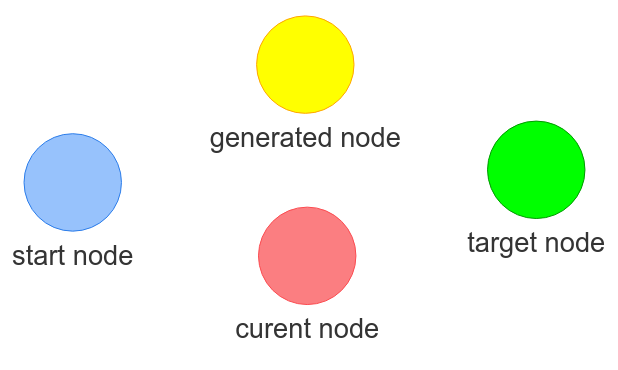
\includegraphics[width=\textwidth]{figures/hgraph_legend_nodes.png}
         \caption{4 nodes used in the HGraph, \textbf{\large Node labels with R:, M: or RM: indicate that the robot is present in the node (R), a model is available (M)}}
     \end{subfigure}
     
     \begin{subfigure}[b]{0.49\textwidth}
         \centering
         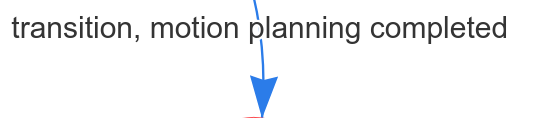
\includegraphics[width=\textwidth]{figures/hgraph_legend_transition1.png}
         \caption{Arrow with solid line}
     \end{subfigure}
    \hfill 
    \begin{subfigure}[b]{0.49\textwidth}
         \centering
         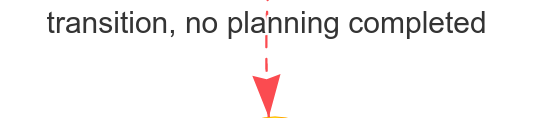
\includegraphics[width=\textwidth]{figures/hgraph_legend_transition2.png}
         \caption{Arrow with dashed line}
     \end{subfigure}
   \caption{HGraph Legend}
    \label{figure: hgraph_legend}
\end{figure}

\begin{figure}[H]
     \centering
     \begin{subfigure}[b]{0.49\textwidth}
         \centering
         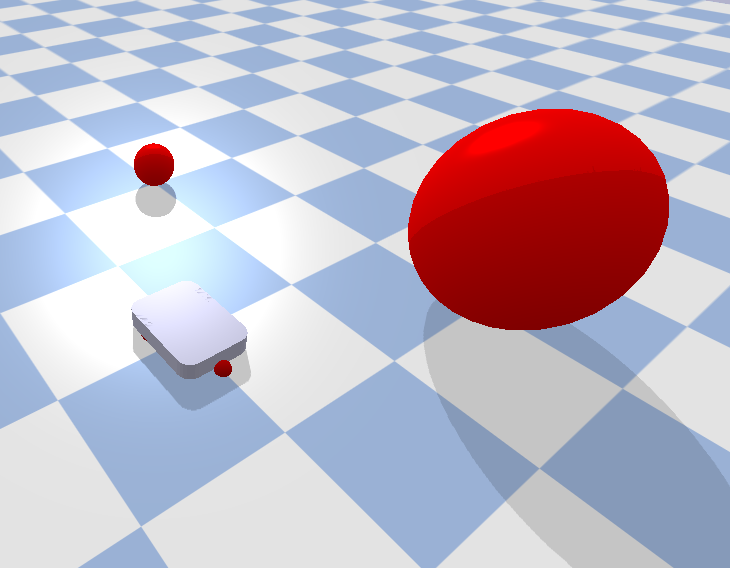
\includegraphics[width=0.75\textwidth]{figures/HGraph_example/task.png}
         \caption{Starting environment, including the robot, the large red sphere to push to the target position indicated with the small red sphere}
     \end{subfigure}
     \hfill
     \begin{subfigure}[b]{0.49\textwidth}
         \centering
         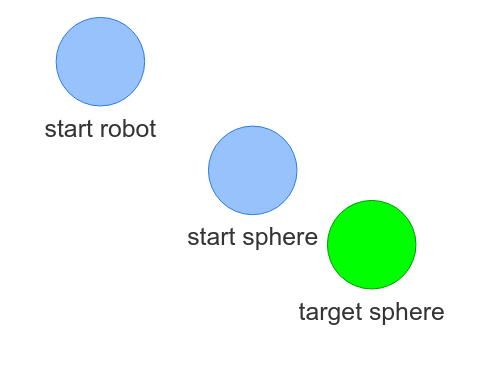
\includegraphics[width=0.95\textwidth]{figures/HGraph_example/1.png}
         \caption{Create initial start and target nodes}
     \end{subfigure}
     \caption{Figure continues on the next page}
\end{figure}

\begin{figure}[H]
\ContinuedFloat
     \begin{subfigure}[b]{0.49\textwidth}
         \centering
         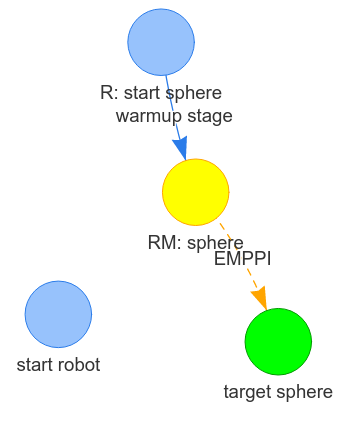
\includegraphics[width=0.95\textwidth]{figures/HGraph_example/2.png}
         \caption{Connect target sphere to starting node sphere with a randomly chosen control methods}
     \end{subfigure}
     \hfill
     \begin{subfigure}[b]{0.49\textwidth}
         \centering
         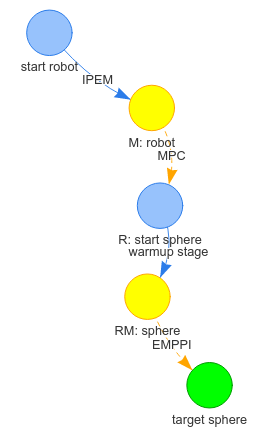
\includegraphics[width=0.95\textwidth]{figures/HGraph_example/3.png}
         \caption{Connect start robot to start sphere because the robot is required for system identification}
     \end{subfigure}
     
     \begin{subfigure}[b]{0.49\textwidth}
         \centering
         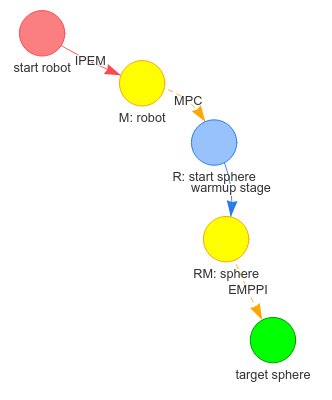
\includegraphics[width=0.95\textwidth]{figures/HGraph_example/4.png}
         \caption{Set start robot as current node}
     \end{subfigure}
     \hfill
     \begin{subfigure}[b]{0.49\textwidth}
         \centering
         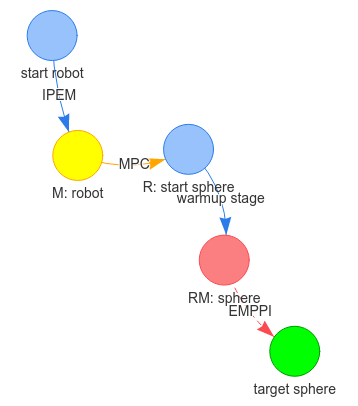
\includegraphics[width=0.95\textwidth]{figures/HGraph_example/5.png}
         \caption{Successfully execute first 3 transitions}
     \end{subfigure}
     
     \caption{The hypothesis graph successfully executing the first hypothesis generated. For the legend, see \cref{figure: hgraph_legend}.}
     \label{figure: example_hgraph}
\end{figure}


